% main.tex
\documentclass[a4paper,oneside,11pt]{memoir}

\usepackage[utf8]{inputenc}
\usepackage[T1]{fontenc}

\usepackage[margin=2.5cm]{geometry}

\usepackage[english]{babel}
\usepackage[hidelinks]{hyperref}

\usepackage{graphicx}
\usepackage{amsmath,amssymb}
\usepackage{listings}
\usepackage{textcomp}
\usepackage{xcolor}

\usepackage{float}
\usepackage{booktabs}
\usepackage{enumitem}

\usepackage{lmodern}
\usepackage{microtype}

\renewcommand{\ttdefault}{pcr}

\lstset{
  basicstyle=\ttfamily,
  keywordstyle=\color{purple}\ttfamily,
  commentstyle=\color{gray}\ttfamily,
  stringstyle=\color{orange}\ttfamily,
  captionpos=b,
  float=tb,
  upquote=true,
}

\chapterstyle{tandh}

\begin{document}

% frontpage.tex
\begin{titlingpage}
\thispagestyle{empty}
\centering

\vspace*{6.5em}

\textsc{\textbf{\huge
    TEK Bachelor’s Project \\[\onelineskip]
    Subject
}}

\vspace{4.5em}

\textsc{\Large
  \setlength{\tabcolsep}{12pt}
  \begin{tabular}[h]{lr}
    Author & name@student.sdu.dk
  \end{tabular}
}

\vspace{2.5em}
\Large
Supervised by Name (name@mmmi.sdu.dk)

\vspace{5em}
\large
Bachelor Project in Software Engineering

\normalsize
\vspace{2em}
\today

\vfill

\noindent
\begin{minipage}[t]{0.60\textwidth}
  \centering
  
\includegraphics[width=0.80\linewidth]{assets/sdu_logo}

  \vspace{1.2em}
  The Maersk Mc-Kinney Moeller Institute
\end{minipage}

\vspace*{1.5em}

\end{titlingpage}


\cleardoublepage
\frontmatter

\input{plain/abstract}

\cleardoublepage
\chapter*{Declaration of AI Usage}
\addcontentsline{toc}{chapter}{Declaration of AI Usage}

Declaration of AI Usage

\cleardoublepage
\input{plain/acknowledgements}

\cleardoublepage
\tableofcontents

\cleardoublepage
\listoffigures

\cleardoublepage
\listoftables

\cleardoublepage
\mainmatter

\input{chapter/1-introduction}
\input{chapter/2-background}
\chapter{Requirements}
\label{chap:requirements}
Requirements
\chapter{System Design}
\label{chap:design}

This chapter sketches the system's structure and a representative
interaction. The two figures below are intentionally generic; they
also double as worked examples of the two diagram source formats
supported by this template (Mermaid and PlantUML, both rendered to
PNG by \texttt{scripts/render-diagrams.sh}).

\section{Architecture overview}
\label{sec:design-architecture}

Figure~\ref{fig:architecture} gives a high-level view of the
components and the direction of data flow between them. The frontend
talks to a REST API, which persists state in a database and enqueues
long-running work for a background worker.

\begin{figure}[H]
    \centering
    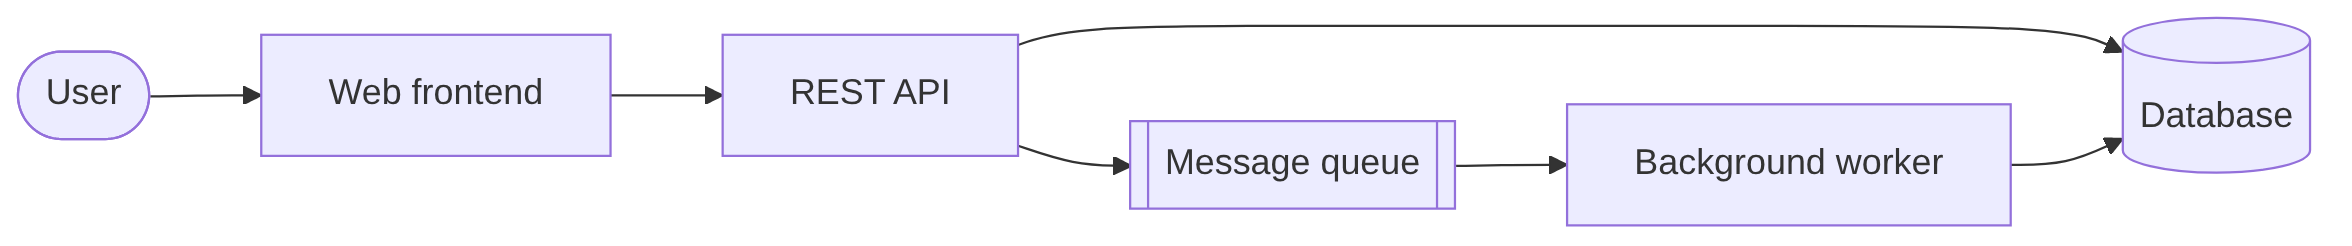
\includegraphics[width=0.85\textwidth]{assets/diagrams/architecture.png}
    \caption{High-level system architecture (Mermaid source:
    \texttt{assets/diagrams/architecture.mmd}).}
    \label{fig:architecture}
\end{figure}

\section{Login flow}
\label{sec:design-login}

Figure~\ref{fig:sequence-login} traces the messages exchanged during a
successful login. The API verifies the supplied password against the
hash retrieved from the database before issuing a session token.

\begin{figure}[H]
    \centering
    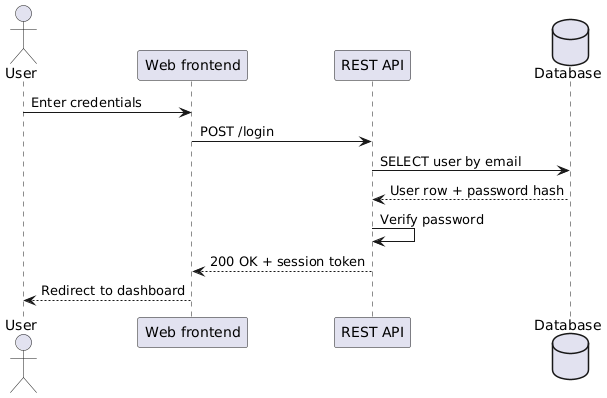
\includegraphics[width=0.85\textwidth]{assets/diagrams/sequence-login.png}
    \caption{Login sequence (PlantUML source:
    \texttt{assets/diagrams/sequence-login.puml}).}
    \label{fig:sequence-login}
\end{figure}

% chap-implementation.tex
\chapter{Implementation}
\label{chap:implementation}

Implementation
% chap-development-process.tex
\chapter{Development Process}
\label{chap:development-process}

Development Process
% chap-conclusion.tex
\chapter{Conclusion}
\label{chap:conclusion}

Conclusion

\appendix
% chap-appendix.tex
\chapter{Appendix}
\label{chap:appendix}

Appendix


\bibliographystyle{unsrt}
\bibliography{mybibliography}

\end{document}
